\chapter{Architektur}
\section{Model View Presenter (MVP)}
Beim Design der Privacy Crash Cam wird schnell deutlich, dass eine strikte Trennung zwischen Datenbank, Applikationslogik und Benutzeroberfläche von Vorteil ist. Neben einer übersichtlichen Unterteilung in einzelne Module unterstützt dieses Vorgehen die Austauschbarkeit der einzelnen Module, deren Wiederverwendbarkeit und Plattformunabhängigkeit. Das Model-View-Presenter-Prinzip realisiert diese Trennung und wird auf auf App und Web interface übertragen.\linebreak\par

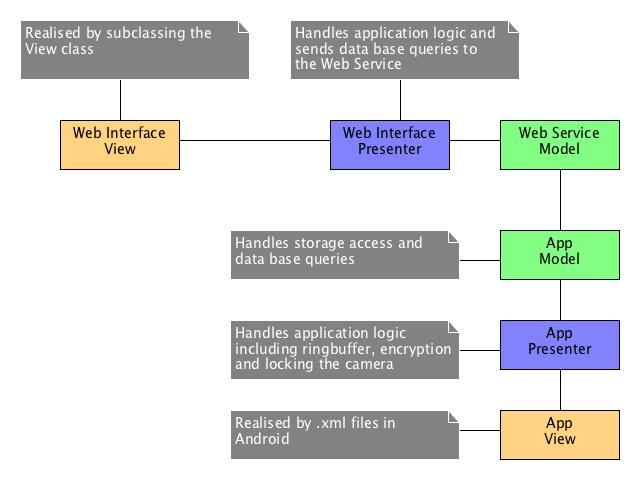
\includegraphics[scale=0.5]{./resources/Diagramme/overview_mvp.jpg}

Die Model-Rolle wird vom Web-Dienst erfüllt. Dieser bietet eine REST API, die sowohl vom Web Interface als auch von der App per HTTP-Anfragen angesprochen wird. Falls weitere Software entwickelt wird, mit der auf die Datenbank zugeriffen werden soll, soll diese ebenfalls auf die selbe API zugrifen können.\linebreak
Darüber hanus besitzt die App ein zusätzliches Model-Modul, das den Speicherzugriff regelt.\linebreak\par

Die Apllikationslogik wird durch die Presenter-Ebene umgesetzt. Hierbei besitzen App und Web Interface eigene Presenter-Module, die an die jeweilige Plattform angepasst sind. Der Presenter handhabt Eingaben durch Nutzer oder Sensoren und koordiniert die darauf folgenden Aktionen, wie das Ändern der Ansicht, Aktualisieren der Ansichten und den Zugriff auf die Model Ebene.\linebreak\par 

Die Rolle der View übernimmt schließlich die GUI. In Android wird diese durch entsprechende XML Dokumente implementiert, in Vaadin durch spezielle Java Klassen die von der Vaadin-Internen Klasse ``UI'' erben. Instanzierung, Manipulation und Navigation erfolgen schließlich durch die Presenter-Ebene, die Bindung erfolgt durch Beobachter und ist bereits durch das jewilige Framework festgelegt.

